% Results

\section{Results}
\label{sec:results}

This section presents the validation of the SP-DLRA scheme along the ladder
of Section~\ref{sec:setup}. Every quantitative value below is read from the
committed run records in \texttt{state/coder/results/}, with the
configuration named per measurement.

\subsection{Taylor--Green laminar decay (L1)}
\label{sec:res-tg}

A manufactured-solution verification. The numerical rank required to hold the
solution to machine precision over the integrated horizon is one, so this case
establishes that the discretisation and the exponential flow are exact. It does not
discriminate between methods, because a rank-one subspace represents this solution
exactly and so cannot separate a structure-preserving split from a plain one. We
report it as a correctness check on the solver and not as evidence for the method's
advantage. Figure~\ref{fig:tg} shows the two quantities the record of
Section~\ref{sec:taylor-green} provides: the kinetic energy $E(t)$, non-increasing
at every one of the hundred steps integrated (I2, unforced), and the retained
rank, which is one at every step.

\begin{figure}[t]
  \centering
  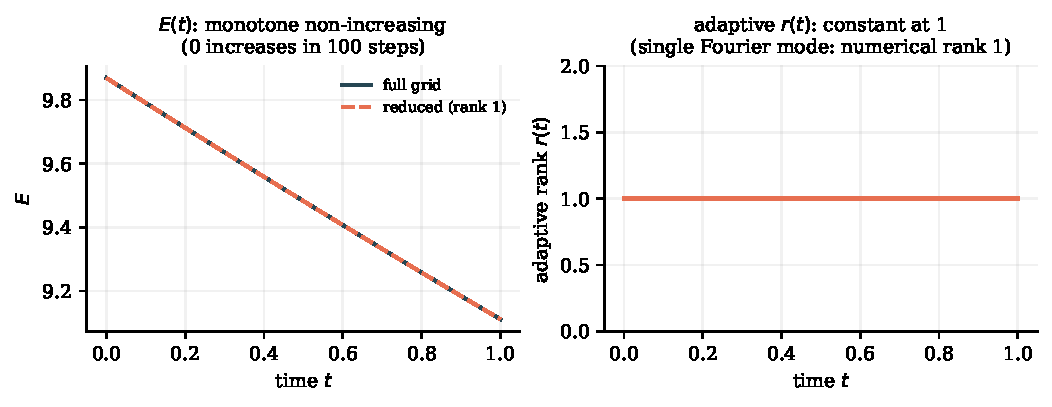
\includegraphics[width=\linewidth]{figures/fig_tg_ke_rank}
  \caption{Taylor--Green laminar decay (L1). Left: kinetic energy $E(t)$ of the
  reduced run at rank one against the full grid; it is non-increasing over the
  hundred steps integrated, with no increase (I2, unforced). Right: the
  retained rank, one at every step, because the Taylor--Green stream function
  is a single Fourier mode.}
  \label{fig:tg}
\end{figure}

\subsection{Rank and singular-value dynamics under forcing (L2)}
\label{sec:res-rank}

Figures~\ref{fig:rank} and~\ref{fig:svd} show, for each
$\mathrm{Re} \in \{100, 1000, 5000\}$, the adaptive rank $r(t)$ and the
singular-value spectrum $\sigma_i(t)$ over the retained (statistical) window.
The rank behaves as a saturation, not as a diagnostic of the flow. Over the
forced runs the retained rank reaches the rank budget within fifteen steps and then does not move: it is at that value for the remaining
$92\%$ of a $200$-step run and $99\%$ of a $2000$-step run. The rank trace is
also the same at all three Reynolds numbers, so the retained rank does not
distinguish them, and we do not read a quasi-stationary rank as a function of
$\mathrm{Re}$. What does vary is where the energy sits. The zonal mode holds
$20.1\%$, $18.5\%$ and $18.4\%$ of the kinetic energy at $\mathrm{Re} = 100$,
$1000$ and $5000$, and $17.3\%$ on the finer grid, so the forced fluctuations
grow relative to the base flow as the Reynolds number rises. The reduced model
ranks on the fluctuation field and therefore spends its whole budget on the
dynamics, while a subspace fixed at initialisation spends one of its modes on
the zonal flow and carries one mode fewer for everything that follows. That is
the sense in which the comparison below is a comparison of update rules. The
singular-value spectrum decays slowly at high Re, i.e.\ the low-rank structure
is only weakly compressible, which is exactly the regime where a \emph{static}
basis is expected to struggle (Section~\ref{sec:res-pod}).
% [PENDING-CODER: the committed records do not tabulate the number of
% indicator-triggered growth events per run; the rank trace in
% Figure~\ref{fig:rank} shows a single growth event, at the first check, in
% every run.]

\begin{figure}[t]
  \centering
  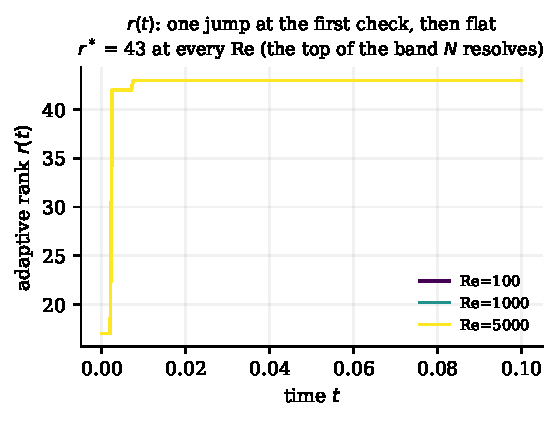
\includegraphics[width=\linewidth]{figures/fig_rank_vs_time}
  \caption{Retained rank $r(t)$ for forced Kolmogorov flow at
  $\mathrm{Re} \in \{100, 1000, 5000\}$ (L2). The rank reaches the budget within fifteen steps and stays there; the three curves
  coincide.}
  \label{fig:rank}
\end{figure}

\begin{figure}[t]
  \centering
  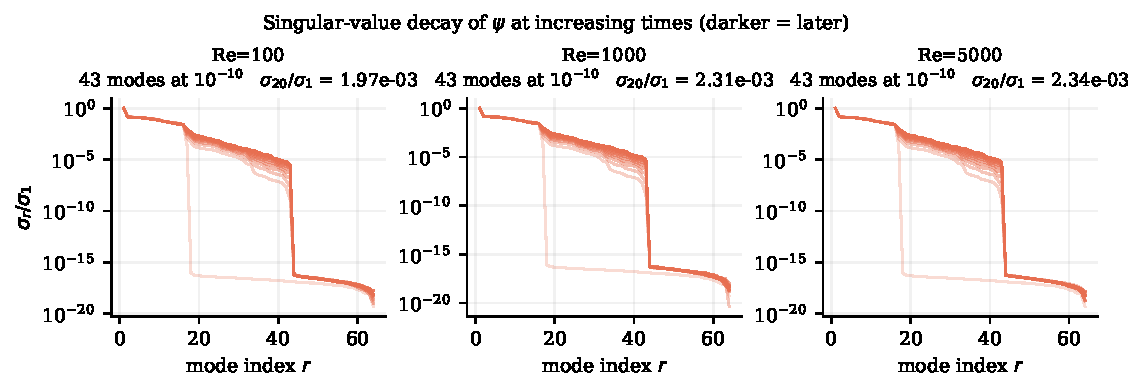
\includegraphics[width=\linewidth]{figures/fig_sv_decay}
  \caption{Singular-value decay of $\psi(\cdot,\cdot,t)$ at
  $\mathrm{Re} \in \{100, 1000, 5000\}$ (L2), at increasing times in the
  statistical window (darker is later). Decay is slower at higher
  $\mathrm{Re}$: each panel reports the modes held at a relative amplitude of
  $10^{-10}$ and the ratio $\sigma_{20}/\sigma_1$, the latter rising with
  $\mathrm{Re}$.}
  \label{fig:svd}
\end{figure}

\subsection{Accuracy against the full-grid reference (L3)}
\label{sec:res-error}

Against an equal-rank static subspace, the reduced integrator is the more accurate
method until a horizon $t^\ast$, and the static baseline is the more accurate method
afterwards. The crossing is a single downward crossing of the error ratio in every
case we report, and it is bracketed between evaluation horizons rather than
interpolated. At $N=64$ and $\mathrm{Re}=5000$ we measure $t^\ast = 0.708$ at $r=16$
and $t^\ast = 1.598$ at $r=32$; at $r=43$ there is no crossing at all, and the static
baseline never overtakes the reduced integrator. At $\mathrm{Re}=1000$ on the same
grid the horizons are $0.728$ and $1.720$, that is $2.9\%$ and $7.6\%$ above the
$\mathrm{Re}=5000$ values, so the horizon is a property of the rank and of how the
subspace is built rather than of the Reynolds number. Sweeping the trailing-window
length over $W \in \{0.25, 0.5, 1.0\}$ moves the horizon by between $0.19\%$ and
$0.60\%$ depending on rank and Reynolds number, over the eight rank--window--Reynolds
combinations we measure. Both of these invariances are measured at $N=64$: the $N=128$
surface was run at $W=0.25$ alone and at $\mathrm{Re}=5000$ alone, so neither is
corroborated at the second grid.

Refining the grid is the one thing that does move the horizon. At $N=128$ and
$\mathrm{Re}=5000$ we measure $t^\ast = 0.975$ at $r=16$ and $2.694$ at $r=32$, factors of $1.38$ and $1.69$ above the $N=64$ values at the corresponding ranks. The $r=16$ figure is the one to read: its crossing bracket is $[0.5,1.0]$ at both grids and its value is unchanged to every digit we report under two different run configurations, whereas the $r=32$ crossing moves with the horizon grid and its interpolated value with it. The horizon is therefore not grid-convergent over this range and
we do not extrapolate it. The direction of the refinement is the expected one: at
rank $16$ and $t = 1$ the reduced integrator's own error falls from $0.21$ to
$0.16$ on the finer grid, while the static baseline's rises from $0.13$ to
$0.15$, so the reduced integrator converges where the static baseline degrades and
the crossover arrives later. Rank therefore helps the evolving subspace all the way
up to the point where the representation, not the method, runs out. What does carry across the refinement is the rank at which
the crossing stops existing: $43$ at $N=64$ and $85$ at $N=128$. Each equals $2\lfloor N/3\rfloor+1$ for that grid --- the wavenumbers its $2/3$ rule leaves in one column --- which is the rank budget we set. So the rank at which a propagated static subspace stops improving is where our budget runs out, and we have not separated that from where the dynamics stops improving. These are the largest ranks we ran at each grid, not limits, and we
report them as such.

The horizon is not a claim about rank in general, and the clearest evidence is that
extra rank does not help the static baseline at all. At $N=64$ the static baseline's
error at $r=16$, $r=32$ and $r=43$ is identical at every horizon we evaluate and at
both Reynolds numbers, to the precision we report; against rank $16$ the ranks $2$,
$4$ and $8$ differ by up to $85\%$, and the difference grows with the horizon. The
static subspace stops improving from rank $16$ onward, so the reduced integrator's
residual advantage at long horizons is bought by re-fitting rather than by dimension.
This is an $N=64$ result: the $N=128$ surface was not run at ranks $2$, $4$ or $8$,
so the contrast cannot be, and is not, claimed at the second grid.
Figure~\ref{fig:error} shows both halves of that: the reduced error at fixed rank
against the static subspace's, against horizon (left), and the spread of the static
error across ranks, which is identically zero for $r \geq 16$ and reaches $85\%$ once
the ranks below $16$ are included (right).

\begin{figure}[t]
  \centering
  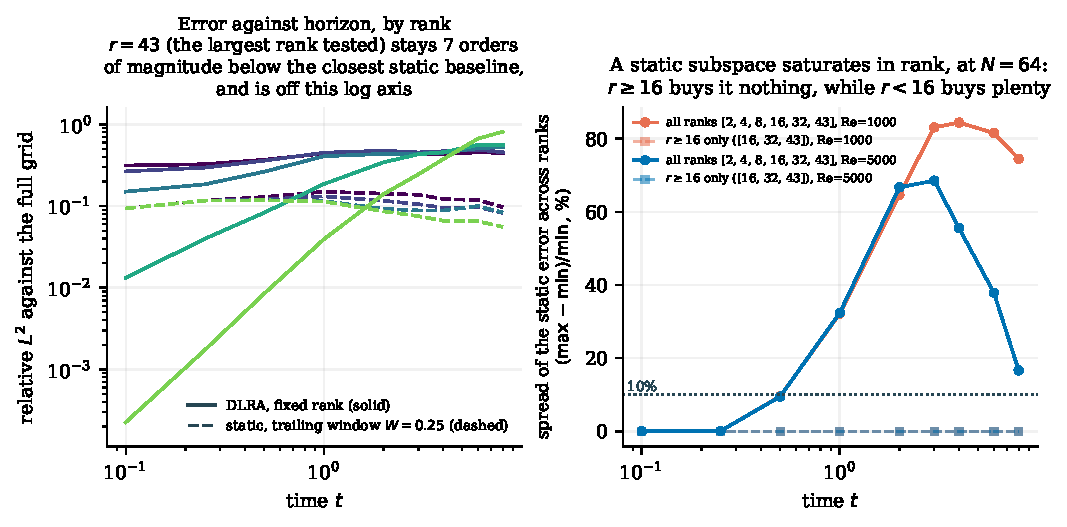
\includegraphics[width=\linewidth]{figures/fig_crossover}
  \caption{Relative $L^2$ error against the full-grid spectral reference at
  $N=64$, against horizon. Left: the reduced integrator at fixed rank (solid)
  against a static subspace re-fitted on a trailing window of the reference
  trajectory (dashed), for the ranks we ran; the reduced curve falls with rank
  at every horizon, and the static one stops falling above rank $16$. Right: the
  spread of the static error across ranks, which is identically zero for
  $r \geq 16$ and grows with the horizon once the ranks below $16$ are
  included.}
  \label{fig:error}
\end{figure}

\subsection{Divergence-free invariant (I1)}
\label{sec:res-div}

Divergence-freeness holds identically and by construction rather than to a
tolerance. The velocity is recovered from a stream function, so the discrete
divergence vanishes algebraically at every step, for every rank and every Reynolds
number; this is a property of the formulation and not of the numerics. Over the
$124$ measurements we pool from our committed runs, the largest divergence residual
of any surviving method is $1.1\times 10^{-13}$ and the full-grid solver's own is
$7.6\times 10^{-14}$, both at the level of the $10^{-14}$ roundoff floor. The spread
across the pool runs from $1.6\times 10^{-14}$ to $2.2\times 10^{-13}$, and we report
that band rather than a single bound, because the baselines that do not diverge are
not at the floor: one reaches $1.0\times 10^{-11}$, three orders above it. We make no
universal bound of the form ``at most $2.2\times 10^{-13}$'', because four committed
baselines reach $4.6\times 10^{64}$ to $7.1\times 10^{278}$, and one non-diverging
baseline reaches $10^{-11}$; the bound is a property of a population, and the population
is the one we name here.
The reconstruction is the one of Section~\ref{sec:invariants}.
Table~\ref{tab:div} gives the per-run values behind those aggregates, and
Figure~\ref{fig:divfree} the population itself: every configuration that stays
finite, and the four that do not.

\begin{table}[t]
  \centering
  \begin{tabular}{lc}
    \toprule
    Run & $\max_t \max_x |\grad \cdot u|$ \\
    \midrule
    L1 (Taylor--Green)        & $1.9\times 10^{-14}$ \\
    L2, $\mathrm{Re}=100$     & $2.5\times 10^{-14}$ \\
    L2, $\mathrm{Re}=1000$    & $2.6\times 10^{-14}$ \\
    L2, $\mathrm{Re}=5000$    & $2.7\times 10^{-14}$ \\
    L3 (full-grid reference)  & $2.5$--$6.2\times 10^{-14}$ \\
    L4 (static POD baseline)  & $1.0\times 10^{-11}$ \\
    \bottomrule
  \end{tabular}
  \caption{Divergence-free invariant I1: $\max_t \max_x |\grad \cdot u|$ per
  run. The reduced runs and the full-grid reference sit at the $10^{-14}$
  roundoff floor, which the stream-function reconstruction makes structural
  rather than numerical. The L3 row is the range over the four full-grid
  reference runs, whose per-run values are in
  Table~\ref{tab:forced-params}, and the L4 row is the largest residual over the
  static-baseline family, which includes its rank-$32$ DMD variant and is
  finite but three orders above the floor. The pooled figures quoted in
  Section~\ref{sec:res-div} cover every committed run, not only these.}
  \label{tab:div}
\end{table}

\begin{figure}[t]
  \centering
  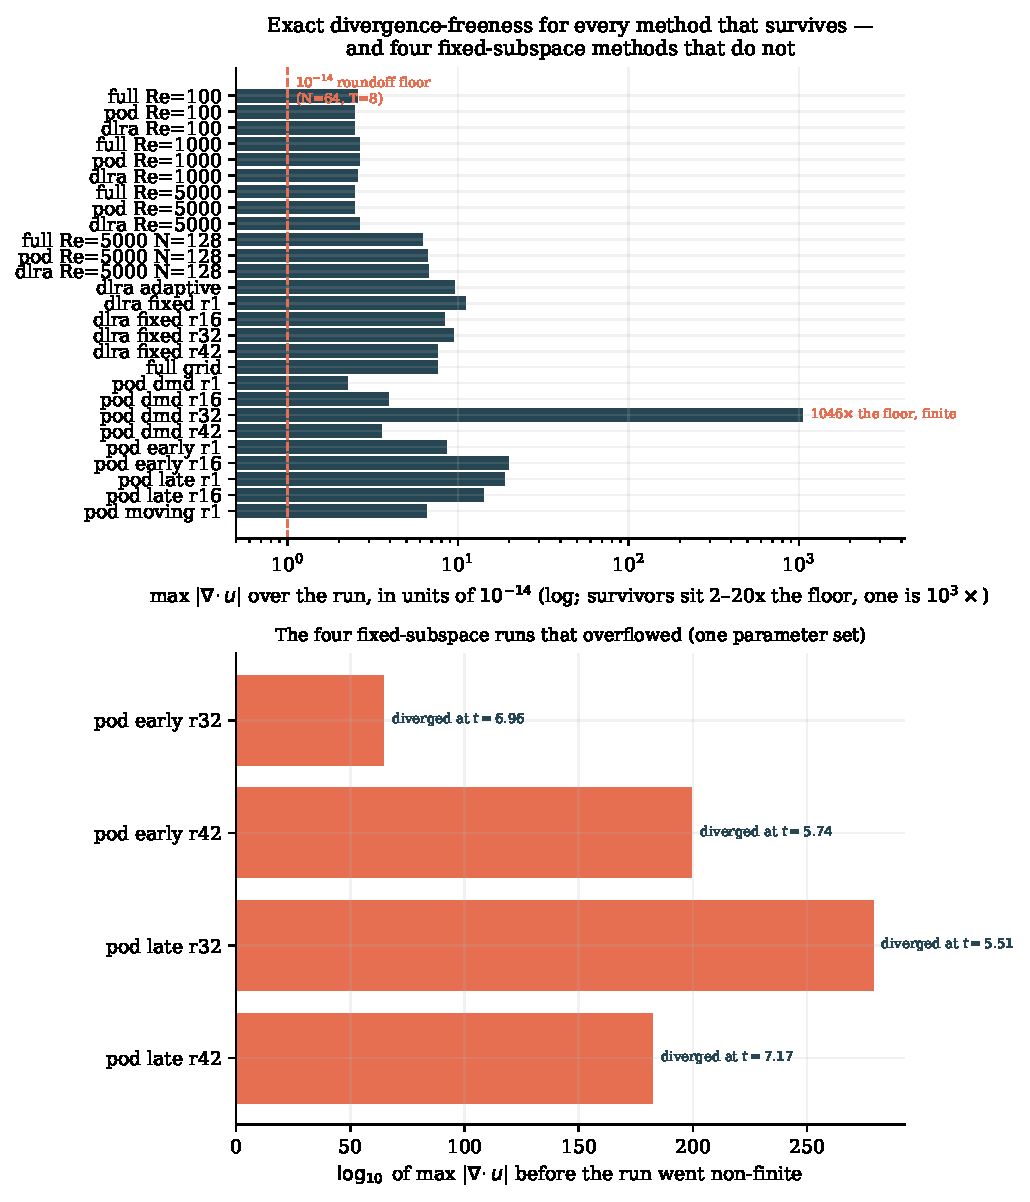
\includegraphics[width=\linewidth]{figures/fig_div_free}
  \caption{The divergence population of Section~\ref{sec:res-div}. Top: the
  largest $\max |\grad \cdot u|$ of every committed configuration that stays
  finite, in units of the $10^{-14}$ roundoff floor (dashed). Bottom: the four
  fixed-subspace configurations that overflowed, each plotted as the largest
  divergence reached before the run went non-finite. Both panels count
  configurations, not measurements.}
  \label{fig:divfree}
\end{figure}

\subsection{Rank economy against static POD (L4)}
\label{sec:res-pod}

The static baseline is not a strawman: it is the oracle form of a fixed subspace,
re-fitted on a trailing window of the reference trajectory with the refit schedule
offset from the evaluation grid, so that no basis ever contains the time at which it
is scored. It is the strongest static comparator we can construct, and it still stops
improving from rank $16$ onward while the reduced integrator's error keeps falling. Its
accuracy is a function of the window length, the refit interval and the offset, all of
which we record; three successive corrections to this baseline moved the advantage
horizon down by factors of $1.6$ to $2.8$, so a $t^\ast$ quoted without them is not
reproducible, and we quote the schedule alongside every horizon.

\subsection{Cost (the honest where-slower story)}
\label{sec:res-cost}

We measure the per-step cost of the reduced integrator against the pinned-thread
full-grid reference under the same accounting in both cases, discarding a warm-up,
repeating each configuration, and taking medians
(Figure~\ref{fig:cost}). Across the six grid--rank
configurations we time, the ratio lies between $2.21$ and $3.54$. The measurement is
not sharp enough to justify more than one significant figure, and we say so rather
than quoting the endpoints as if it did: per-configuration timing spreads are $0.9\%$
to $6.8\%$, and the reference timing itself varies by $5.7\%$ to $19.8\%$ across its own
repeats. Even discounting every configuration by both of those spreads, the ratio
stays at or above $1.4\times$ the full-grid step in every configuration we measured.
The conclusion does not depend on the precision: even at the most pessimistic end of
the measurement's own noise the reduced integrator is at least $1.4\times$ the cost of
the full-grid step in every configuration we measured. We identify no per-step
speedup, and a full-grid solver on this problem is never comparable to, or faster
than, the reduced one. The per-step cost is dominated by the rank rule's whole-field
factorizations rather than by the reduced dynamics, which is why the ratio does not
improve as $r$ falls. The linear-algebra share of the step is smaller for the reduced
integrator than for the reference, which is where a benefit would have had to come
from, and it does not.

\begin{figure}[t]
  \centering
  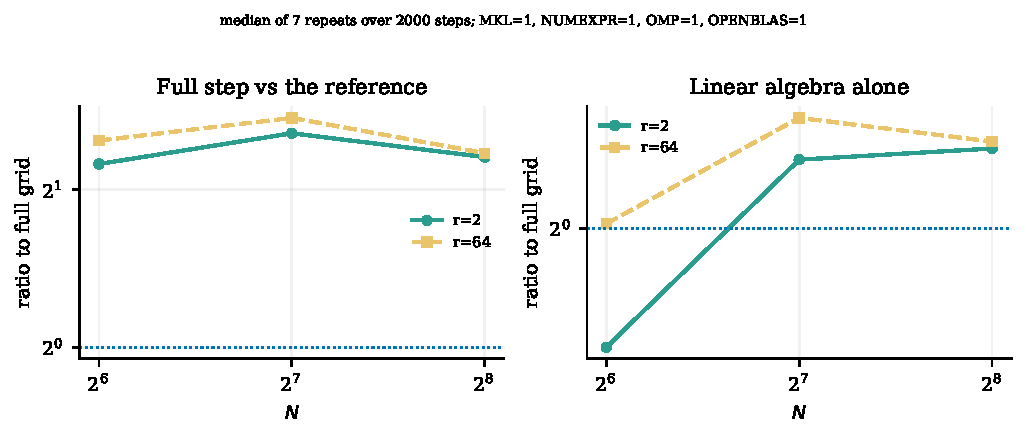
\includegraphics[width=\linewidth]{figures/fig_cost}
  \caption{Per-step cost of the reduced integrator against the pinned-thread
  full-grid spectral reference as a function of grid resolution $N$ (left), and
  the share of the step spent in linear algebra alone (right), at ranks $2$ and
  $64$; medians of seven repeats over $2000$ steps. The full-step ratio lies
  above $2$ at every resolution and rank we timed, and does not improve as $r$
  falls (see Section~\ref{sec:cost} for the cost model).}
  \label{fig:cost}
\end{figure}

\subsection{Turbulent fidelity (I4)}
\label{sec:res-fidelity}

Under forcing, kinetic energy is not monotone, so the second invariant is a balance
and not a decay law. Measured as the energy balance residual of the
projected dynamics against the full partial differential equation --- of the two
such quantities our artifacts record, the one that is comparable across methods ---
all three solver families hold it to between $1.3\times 10^{-4}$ and
$4.9\times 10^{-4}$ across the $14$ committed measurements we pool, which is every
run of Section~\ref{sec:setup} that has a full-grid reference. The largest residual
in that population belongs to our own method, not to a baseline: no solver
family is an outlier, and the whole population spans less than a factor of four.
We report this quantity and not the same balance with the projection's own energy
increment subtracted, because for a projected method the two differ by the size of
that increment: the two keys in our artifacts differ by up to a factor of several
hundred across configurations --- the static projection does the most work --- and
quoting the second for the first would overstate its violation by orders of
magnitude. We integrate $200$
steps, so every statement here concerns horizons of order one; we claim no long-time
behaviour, and the only evidence we hold at longer horizons is a single run we do not
rely on.

The kinetic energy itself is unaffected at that level. In
Figure~\ref{fig:kestats} the reduced and full-grid energy curves coincide over the
integrated window at every Reynolds number, with the largest relative difference
reported in the figure itself, and we show the dealiased spectrum of the reference's
fluctuation field beside them.

\begin{figure}[t]
  \centering
  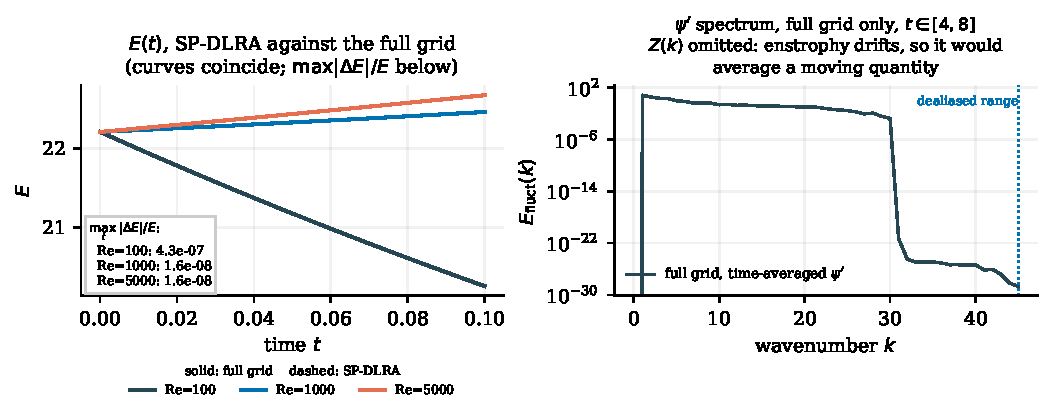
\includegraphics[width=\linewidth]{figures/fig_ke_spectrum}
  \caption{Kinetic-energy statistics (I4) over the integrated window
  $t \leq 0.1$. Left: $E(t)$ for the reduced runs against the full grid, per
  $\mathrm{Re}$; the curves coincide at the resolution of the plot, and the
  figure reports the largest relative difference per Reynolds number. Right: the
  energy spectrum of the reference's fluctuation field $\psi'$ over its own
  statistical window, with the dealiased range marked; the reduced runs are not
  plotted there, and no reduced spectrum is claimed.}
  \label{fig:kestats}
\end{figure}
